\section{am::lambda::condition Struct Reference}
\label{structam_1_1lambda_1_1condition}\index{am::lambda::condition@{am::lambda::condition}}
Predicate.  


{\tt \#include $<$lambda.hpp$>$}

Inherits {\bf am::lambda::detail::lambda\_\-op\_\-tag}.

Inheritance diagram for am::lambda::condition:\begin{figure}[H]
\begin{center}
\leavevmode
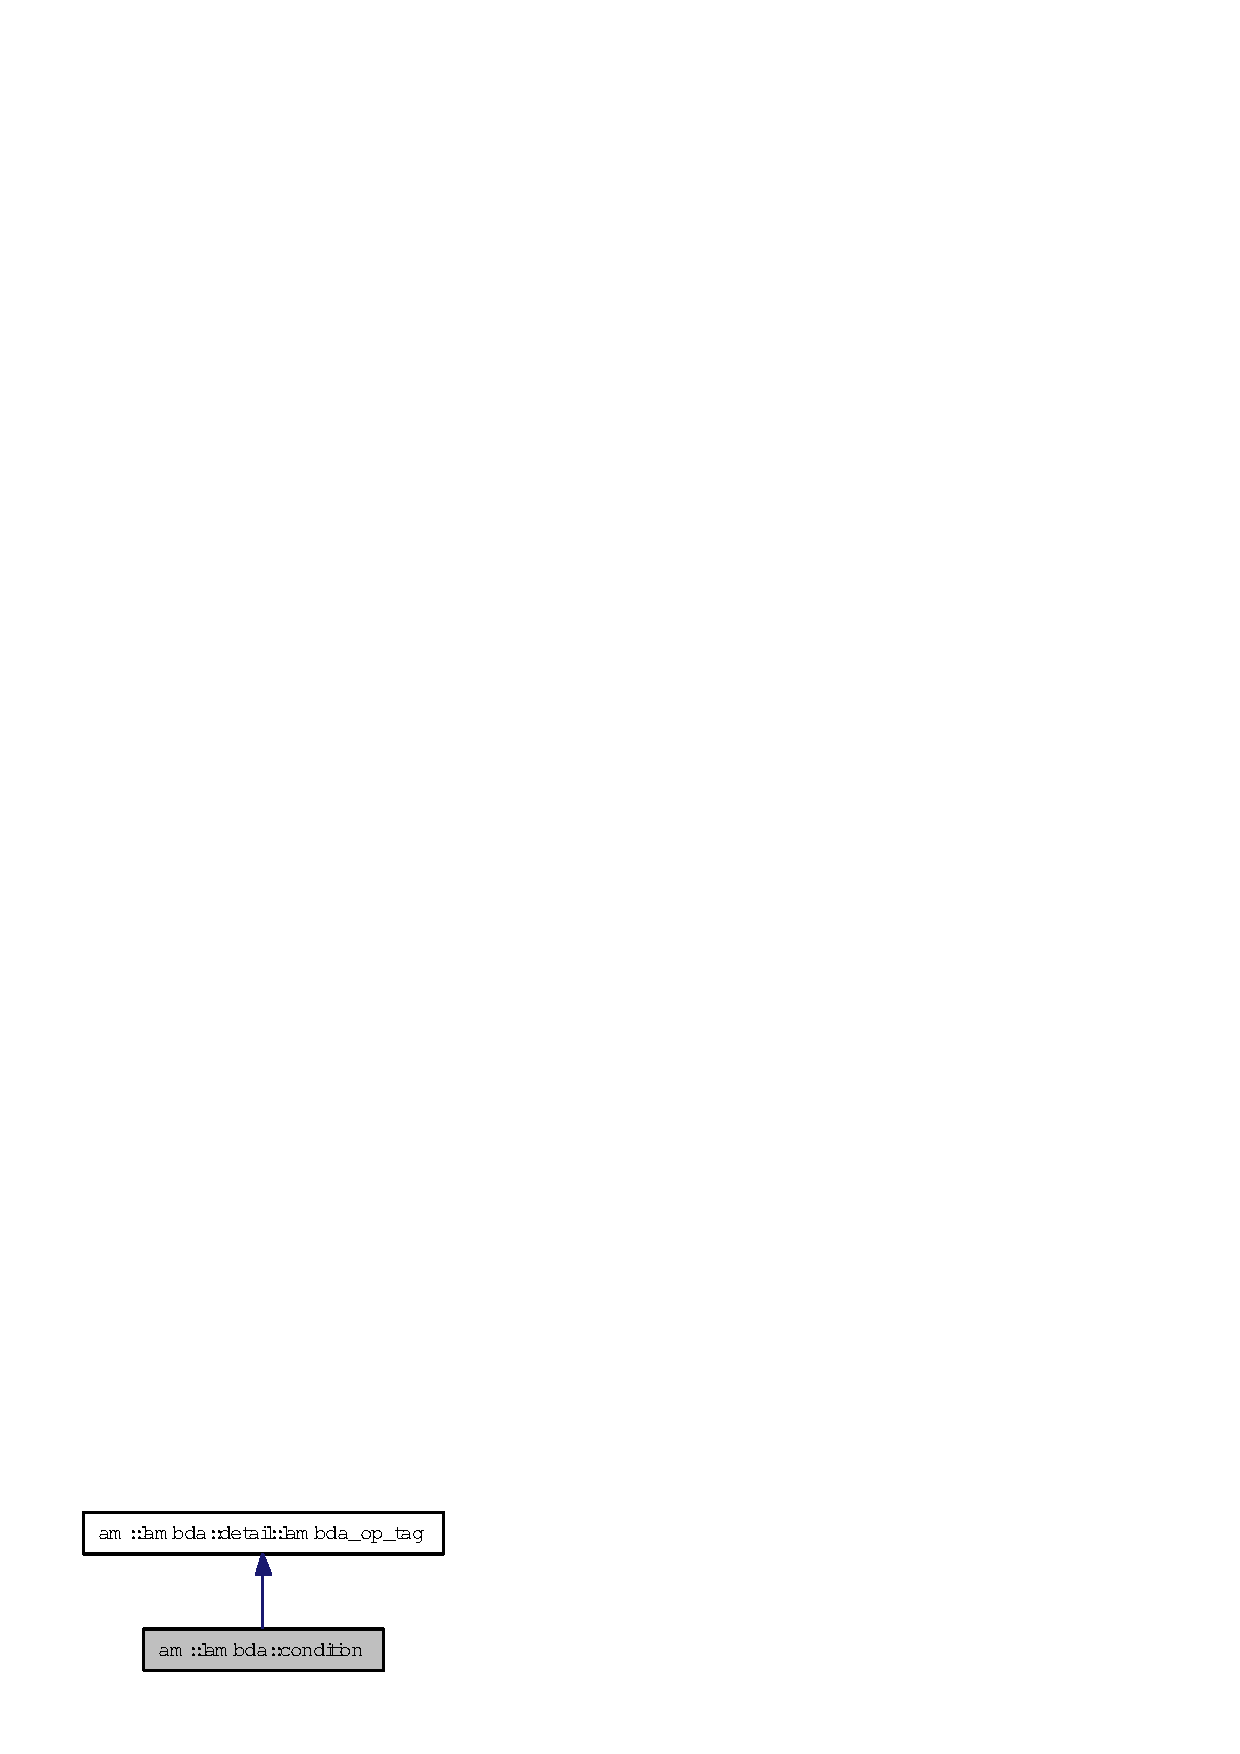
\includegraphics[width=108pt]{structam_1_1lambda_1_1condition__inherit__graph}
\end{center}
\end{figure}
Collaboration diagram for am::lambda::condition:\begin{figure}[H]
\begin{center}
\leavevmode
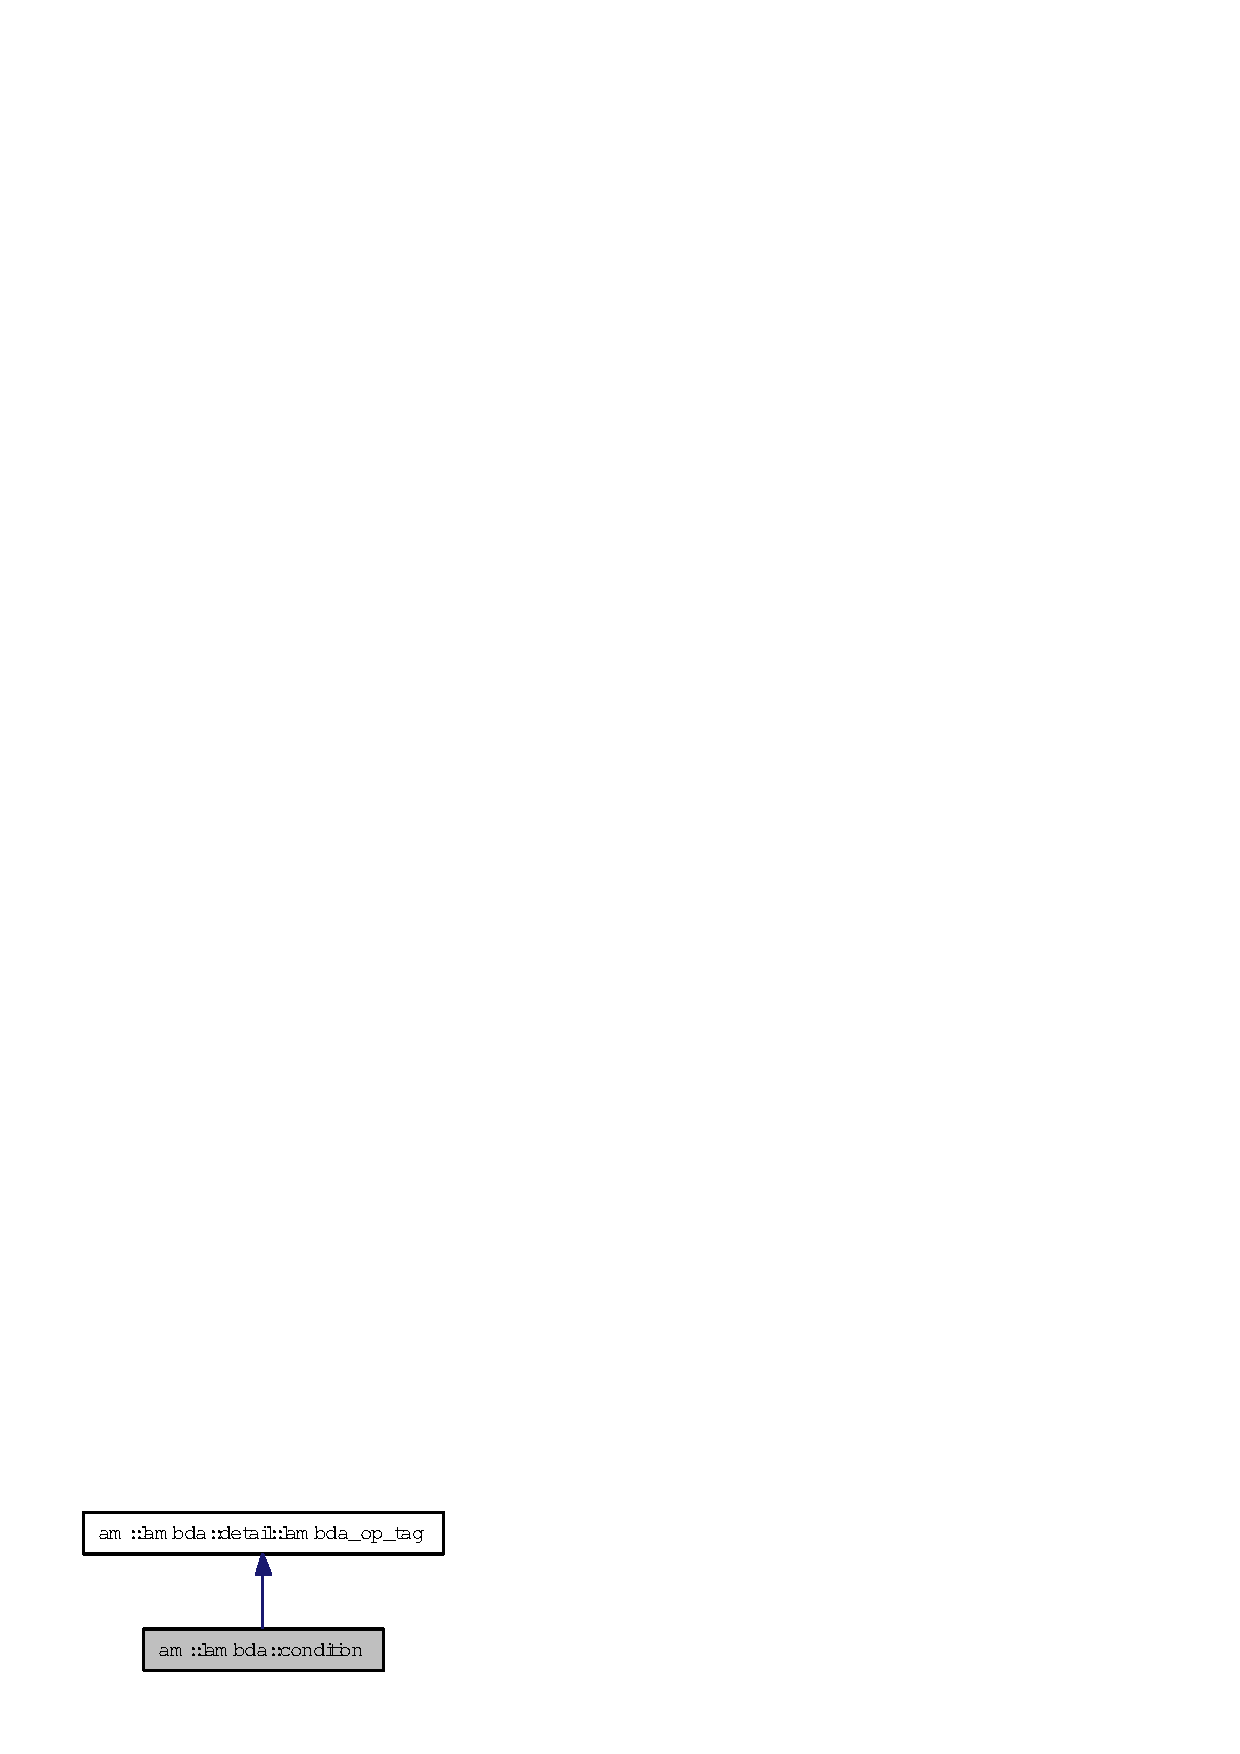
\includegraphics[width=108pt]{structam_1_1lambda_1_1condition__coll__graph}
\end{center}
\end{figure}
\subsection*{Public Member Functions}
\begin{CompactItemize}
\item 
\textbf{condition} (bool b)\label{structam_1_1lambda_1_1condition_e40f01ee1d36564ae8fc2741d810ee67}

\item 
template$<$class T1, class T2, class T3$>$ bool \textbf{operator()} (T1, T2, T3) const\label{structam_1_1lambda_1_1condition_01b6a3632c9427e5751d25553c0b7299}

\item 
template$<$class T1, class T2$>$ bool \textbf{operator()} (T1, T2) const\label{structam_1_1lambda_1_1condition_7c9b36804edcb13cd6d92de83557abd9}

\item 
template$<$class T1$>$ bool \textbf{operator()} (T1) const\label{structam_1_1lambda_1_1condition_08a614f29cafff6959b43fc64485e40b}

\item 
bool \textbf{operator()} () const\label{structam_1_1lambda_1_1condition_19e3c55b10f5c5edf3fdf099d26a365c}

\end{CompactItemize}
\subsection*{Public Attributes}
\begin{CompactItemize}
\item 
bool \textbf{b\_\-}\label{structam_1_1lambda_1_1condition_19014c303208f7d24845652348737106}

\end{CompactItemize}


\subsection{Detailed Description}
Predicate. 

Convert a boolean expression into null-nary or unary predicate. 



The documentation for this struct was generated from the following file:\begin{CompactItemize}
\item 
{\bf lambda.hpp}\end{CompactItemize}
